\section{Babbling and phonetic imitation on the iCub}

IST has continued the development of the architecture for speech
development. The role of the architecture is to allow the robot to
simultaneously develop speech perception and production, and learn how
to perceive and produce simple words. The learning is done through a
combination of babbling and imitation. Using this approach the robot
has currently been able to learn to perceive and produce single
phonemes such as vowels and simple consonants. 
\begin{figure}
\centering
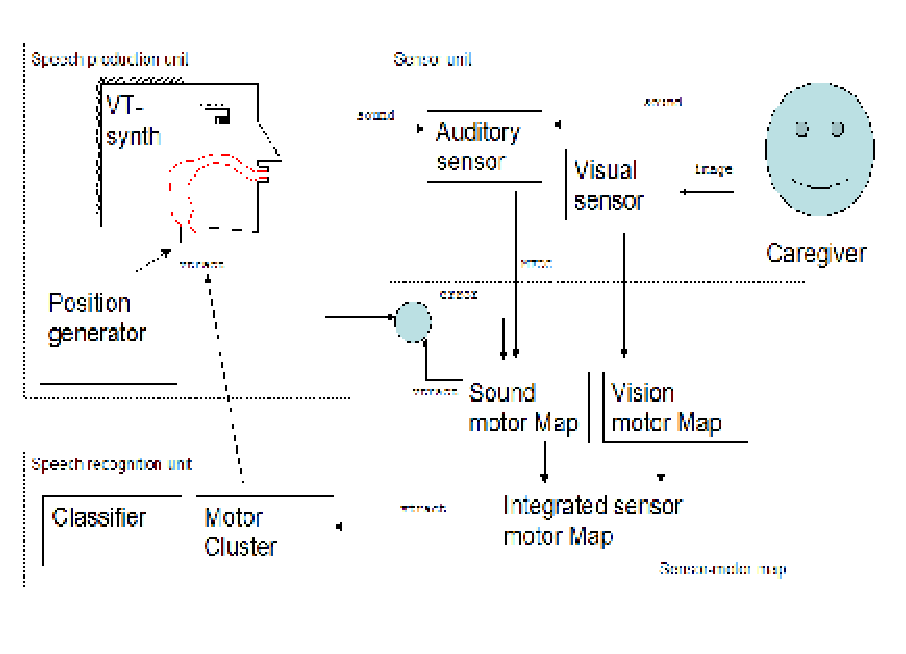
\includegraphics[width=0.8\textwidth]{include/babbling/images/arch.eps}
\caption{System architecture for speech development.}
\label{fig:babbling:arch}
\end{figure}

\subsection{System architecture}
The current version of the architecture includes a speech production
unit, a sensor unit, a sensor-motor map and a speech recognition unit,
Figure~\ref{fig:babbling:arch}.

The speech production unit is responsible for moving the lips and
producing sound. The vocal tract is simulated using vtcalcs developed
by Maeda [ref]. This model has six parameters that can be used to
control the movements of the vocal tract. One parameter is used for
the controlling the position of the yaw, one for the protrusion of the
lips, one for lip opening, and three parameters for controlling the
position of the tongue. A synthesizer converts the vocal tract
positions into sound. While the synthesizer works well for vowel-like
sounds, it is unable to produce fricatives sounds and can therefor
only produce a limited set of consonants.

The sensor unit contains two sensors, an auditory sensor unit and a
visual sensor unit. The auditory sensor records sound and windows the
sound signal into 30 ms frames with 50\% overlap. For each frame 12
Mel frequency cepstral coefficients (MFCC) are calculated for each
frame. The visual sensor unit takes images from a video stream and,
given that it can see the subject that is talking, calculates the
openess of the mouth. The Mel coefficients and the openess of the
mouth are normalized and sent to the sensor-motor map.

The sensor-motor map contains two separate artificial neural networks
that maps the respecitve sensor output from the auditory and visual
sensor to the robots motor representation, i.e. the six parameters in
Maedas model. The sound-motor map is the more complex of the two maps
and uses a neural network with 20 hidden neurons, while the
vision-motor map only uses a single neuron. The outputs from the two
maps are then weighted together. The weight is currently set by hand.

The speech recognition unit consists of a cluster and a
classifier. The cluster contains motor positions for each of the
phonemes that the robot has leart. The classifier simply measures the
distance between a given motor position and each position that has
been stored in the cluster and classify the position as the nearest
neighboor.
 
\subsection{Babbling and imitation}
The robot uses a combination of babbling and imitation to learn how to
recognize and produce speech. These methods are inspired by the way
children develop their speech. The babbling is important to create an
initial map between the produced sound and the robots motor positions
of the robot's vocal tract. However, to be able to map speech from a
human speaker the robot has to interact with a caregiver. This is done
by having the caregiver immitating the robot. To be able to learn
phonemes we do the opposite and let the robot immitade the caregiver.

The babbling behavior is realised by the position generator by taking
a pair of either existing positions in the motor cluster (given that
such positions exists) or randomly chosen positions. A trajectory is
then created between the two positions. Along the trajectory a number
of new positions are created and sent to the speech production
unit. The produced sound is then fed into the auditory sensor unit
that calculates the MFCC and passes these to the sound-motor-map. The
sound-motor-map finally tries to map the MFCC back to the original
articulator position vector and compares the result with the output
from the position generator. The error between the mapped and the
correct positions is the used to update the map using a
back-propagation algorithm.

By having a human caregiver listening to the output of the robot and
repeating the same utterance with his or her own voice, the robot is
able to map not only the synthesized speech, but also the voice of the
caregiver, back to the motor positions. In the same time it can also
learn its vision-motor map by mapping the calculated mouth opening of
the human and comparing it with its own motor parameters. By having
several caregivers immitating the robot we are able to gain some
amount of speaker invariance.

Finally we let the robot immitate the caregiver. If the caregiver is
happy with the given response he or she gives positive feedback to the
robot which causes the robot to store the motor positions in the motor
cluster. These positions can later be used to drive further babbling
and interaction with the caregiver.

We performed two experiments using the architecture with babbling and
imitation as described above. In the first experiment we learn the
robot 9 portuguese vowels and especially investigate the effect of the
visual features for vowel recognition. In the second experiments we
teach the robot some simple consonants and again study the effect of
using vision for recognition. We also study the well know Mc Gurk
effect which can be expected when combining visual and auditory
features.

\subsection{Experimental results}
Using the described method of babbling and imitation the iCub has been
able to learn a number of portuguese vowels and a few consonants. The
vocal tract positions used by the robot to produce those phonemes
resemples the positions used by a human speaker. The positions used to
pronounce nine portuguese vowels are shown in Figure~\ref{fig:babbling:positions}, and the
positions used to pronounce the consonants /b/, /d/ and /g/ are shown
in Figure~\ref{fig:babbling:cardinal}.

IST also done some initial test on how well the robot is able to
recognize those vowels when pronounced by different speakers. A total
of 14 speakers (seven males and seven females) were recorded while
reading words that included the vowels. The vowels from seven of the
speakers were used as a training set and the vowels from the other
seven were used as test data. After learning the maps using random
babbling the recognition rate for the vowels in the test set was as
low as 17.5\%. After having the seven humans in the training data
immitating the robot, but only using the auditory information, the
recognition rate reached 57.7\%. Finally by using both auditory and
visual data during training and testing, the recognition rate got up
to 63.3\%.

\begin{figure}
\centering
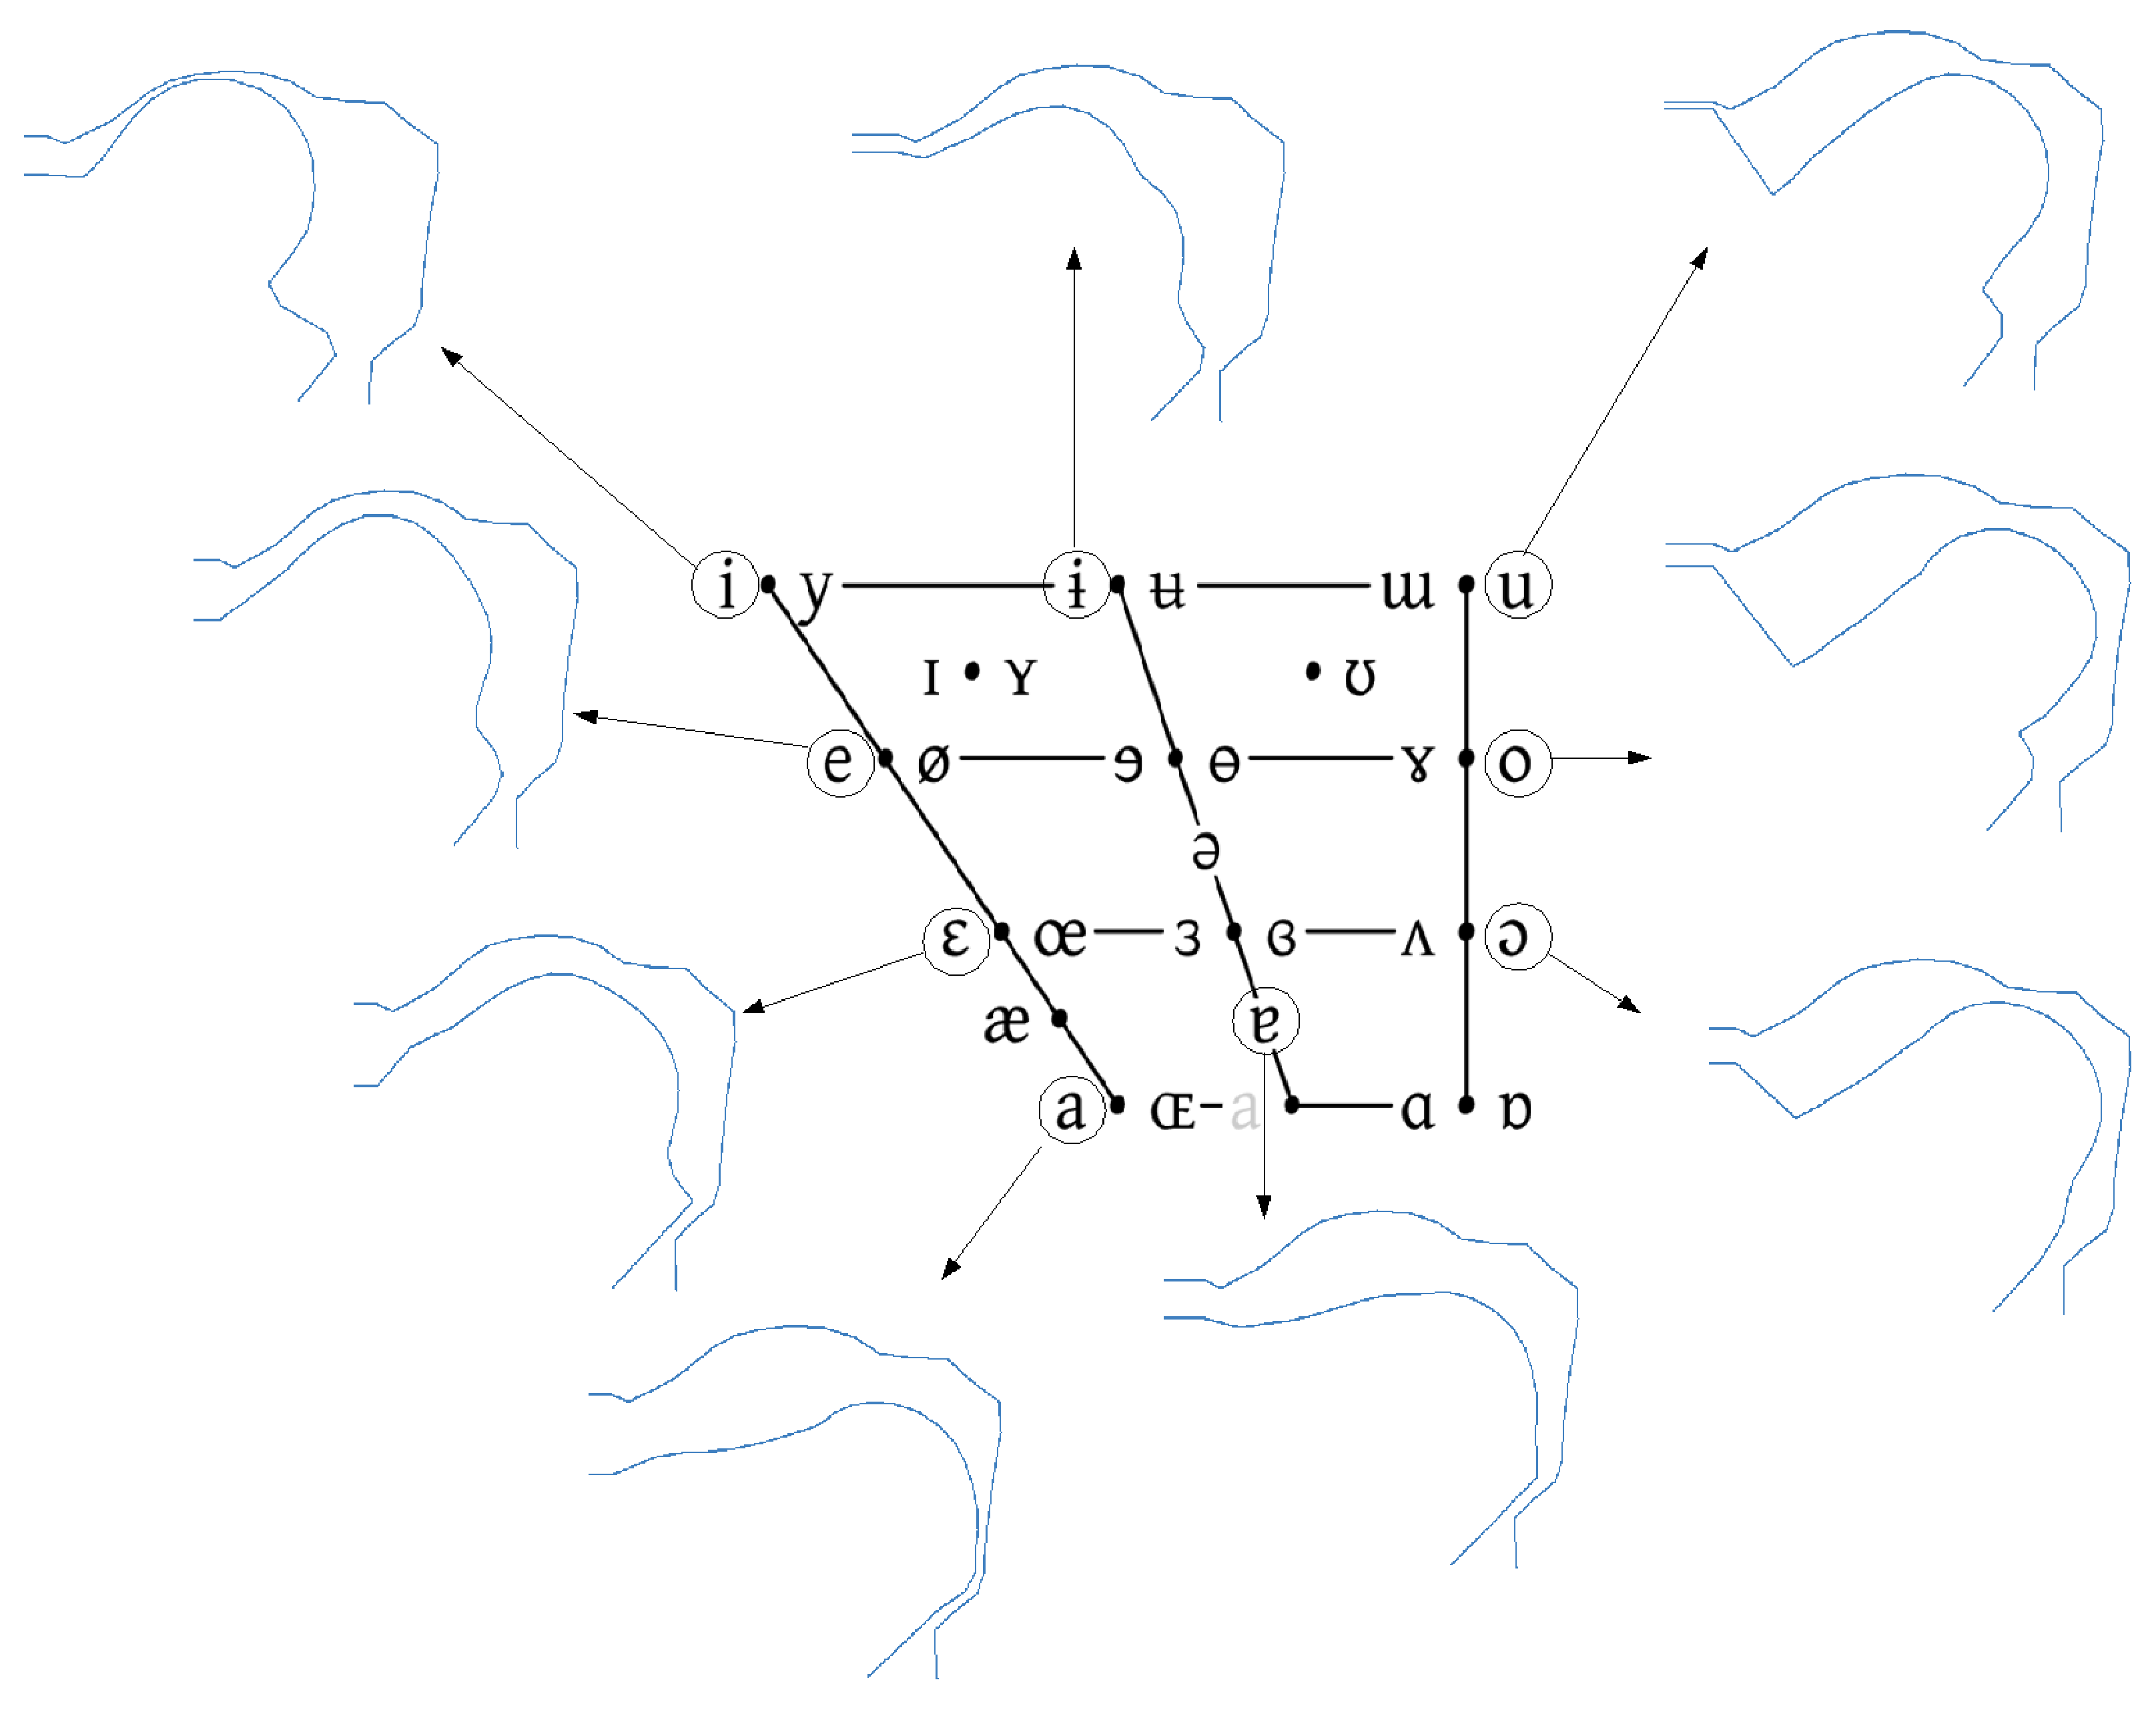
\includegraphics[width=0.8\textwidth]{include/babbling/images/vowels.eps}
% Figure 3 
\caption{Articulator positions used by the robot for the
  Portuguese vowels. In the center we show the positions of the vowels
  in the International Phonetic Alphabet (IPA). The vertical axis in
  the IPA corresponds to the vertical position of the tongue and the
  horisontal axis to the front-back position when the vowel is
  pronounced by a human speaker. For the simulated articulator
  positions used by the robot the upper line corresponds to the soft
  palate and the lower line to the tongue. There is a good correlation
  between how the robot and a human articulate the vowels.}
\label{fig:babbling:positions}
\end{figure}

\begin{figure}
\centering

\includegraphics[width=0.8\textwidth]{include/babbling/images/cardinal.eps}
% Figure 4 
\caption{Articulator positions for /b/, /d/, and /g/.}
\label{fig:babbling:cardinal}
\end{figure}


\endinput
